\documentclass[14pt]{article}
% Эта строка — комментарий, она не будет показана в выходном файле
\usepackage{ucs}
\usepackage[utf8x]{inputenc} % Включаем поддержку UTF8
\usepackage[russian]{babel}  % Включаем пакет для поддержки русского языка
\usepackage{amsmath}
\usepackage{amssymb}
\usepackage{mathtools}
\usepackage{hyperref}

\hoffset=0mm
\voffset=0mm
\textwidth=160mm        % ширина текста
\oddsidemargin=0mm   % левое поле 25.4 - 5.4 = 20 мм
\textheight=240mm       % высота текста 297 (A4) - 40
\topmargin=-15.4mm      % верхнее поле (10мм)
\headheight=5mm      % место для колонтитула
\headsep=5mm          % отступ после колонтитула
\footskip=8mm         % отступ до нижнего колонтитула

\title{
\textbf{Метрическая Задача Коммивояжера} 
}

\date{\today}
\author{Миллер Сергей}

\begin{document}
    \maketitle
    \paragraph{\large{1. Введение}}
    \begin{flushleft}
   Проблемой коммивояжера (поскольку этот вопрос возникает у каждого почтальона, в частности, её решают многие путешественники) называют задачу поиска кратчайшего пути между конечным множеством мест, расстояние между которыми известно. 
   В данной работе рассматривается метрический случай данной задачи.
    В частности, эта задача  находит применение при сверлении отверстий в печатных платах, когда станок должен сделать больше отверстий за наименьшее время и может перемещать сверло в обоих направлениях для перехода от одного отверстия к следующему.
    \end{flushleft}  
    
    \paragraph{\large{2. Поставленные вопросы}}
    \begin{itemize}
    \item  Несуществование полиномиального алгоритма для стандартной задачи коммивояжера, дающего константное приближение, если $\mathbf{P} \neq \mathbf{NP}$.
    \item Построение алгоритма для метрической задачи, дающего 2-приближение на основе остовного дерева.
    \item Построение алгоритма для метрической задачи, дающего 1.5-приближение на основе остовного дерева и паросочетания.
    \item Имплементирование алгоритма, дающего 1.5-приближение.
    \end{itemize}

    \paragraph{\large{3. Теория и определения}}\mbox{}\\

    Сформулируем несколько известных определений и вспомним некоторые факты из курса сложности вычислений.

    \textbf{Определение 1.} Цикл в графе $G$ называется \textit{гамильтоновым}, если проходит через все вершины в $G$ ровно по одному разу.

    \textbf{Определение 2.}  Подграф  $H \subset G$ в графе $G = (V,E)$ называется \textit{остовным деревом}, если $H$ - дерево и $V(H) = V(G)$.

    \textbf{Определение 3.} Граф $G = (V,E)$ c определенной на его ребрах функцией весов  $w: E \to \mathbb{R}_{+}$ называется \textit{метрическим}, если $\forall x,y,z \in V: w(x,z) \leq w(x,y) + w(y,z)$

    \textbf{Определение 4.} Язык $A$ называется $\mathbf{NP}$-\textit{полным}, если для каждого языка $B \in \mathbf{NP}$   существует полиномиально вычислимая функция $f_B:\{0,1\}^* \to \{0,1\}^*$ такая, что $\forall x \in \{0,1\}^*: x \in A \iff f_B(x) \in B$.

    \textbf{Определение 5.} \textit{(Метрической) Задачей коммивояжера} называется язык пар 

     $L = \{(G,k)|$ в (метрическом) полном графе $G$, c заданными весами ребер $w$, существует гамильтонов цикл веса не более  $k\}$.

    Неформально, эту задачу можно рассматривать как задачу поиска гамильтонова цикла наименьшего веса в полном (метрическом) взвешенном графе $G$.

    \textbf{Определение 6.} Полиномиальный алгоритм дает $c$-приближение, если результат работы алгоритма отличается от верного не более чем в $c$ раз.

    Из курса сложности вычислений знаем, что язык 

    $\text{HAMCYCLE}=\{G| \text{в графе G сущестует гамильтонов цикл}\}$ - \textbf{NP} - полный.
    \newpage

    \paragraph{\large{4. Несуществование алгоритма дающего $c$-приближение для стандартоной задачи коммивояжера}}\mbox{}\\

    \textbf{Теорема 1} \textit{Для стандартной задачи коммивояжера не существует алгоритма, работающего за полиномиальное время и дающего константное приближение, если $\mathbf{P} \neq \mathbf{NP}$.}

    \textit{Доказательство}. Пусть такой алгоритм существует, и дает $c$-приближение, тогда покажем как с его помощью определить принадлежность графа $G$ к языку HAMCYCLE. Рассмотрим произвольный граф $G = (V,E)$. Достроим $G$ до полного взвешенного графа $\hat{G}$ следующим образом: ребрам из $E$ сопоставим вес 1, а всем остальным - $nc + 1$, где $n = |V|$ - количество вершин в $G$. Применим найденный алгоритм к $\hat{G}$. На выходе получим какой-то гамильтонов цикл веса $w$.

     Теперь если $w \leq cn$, то на самом деле кратчайший цикл имеет вес не больше $w$, а это значит, что все ребра в нем имеют вес ровно 1, то есть присутствовали также и в исходном графе $G$, то есть в нем был гамиьтонов цикл. 

     Если же наоборот $w > cn$, то это означает, что наименьший гамильтонов цикл имеет вес $w_0 >= \frac{w}{c} > n$, то есть обязан содержать хотя бы одно ребро веса $cn+1$, которого не было в $G$.

     В итоге с помощью полиномиального алгоритма научились решать \textbf{NP}-полную задачу, откуда следует, что $\mathbf{P} = \mathbf{NP}$. А это противоречит заданному условию. $\Box$


    \paragraph{\large{5. 2-приближение для метрической задачи}}\mbox{}\\

    \textbf{Теорема 2}\textit{ Для метрической задачи коммивояжера существует полиномиальный алгоритм, дающий 2-приближение.}

    \textit{Доказательство}. Построим этот алгоритм явно на основе остовного дерева. Для построения алгоритма докажем вспомогательную лемму.

    \textbf{Лемма 1}. \textit{Пусть $G = (V,E)$ - полный взвешенный метрический граф и $C$ - цикл в $G$ веса $w_0$, проходящий через все вершины в $G$. Тогда граф $G$ содержит гамильтонов цикл веса не более $w_0$.}

    \textit{Доказательство леммы}. Пусть $C = \{v_0, \dots v_k\}$. Заметим, что все вершины $G$ встречаются в $C$. Тогда оставим в $C$ вершины только в позициях своего первого вхождения. Получим некоторую перестановку вершин из $G$, которой соответствует гамильтонов цикл $\hat{C}$ в $G$. Легко видеть, что его вес не больше $w_0$, так как при выкидывании вершин из $C$, фактически произвелась замена ребер $(v_k, v_{k+1}), (v_{k+1}, v_{k+2}), \dots (v_{m-1}, v_m)$ на одно ребро $(v_k, v_m)$. Но в силу неравенства треугольника: $w(v_k,v_m) \leq w(v_k,v_{k+1}) + w(v_{k+1}, v_m) \leq \dots \leq (v_k, v_{k+1}) + (v_{k+1}, v_{k+2}) + \dots + (v_{m-1}, v_m)$. Откуда следует, что $w(\hat{C}) \leq w(C)$. То есть в графе $G$ найдется гамильтонов цикл $\hat{C}$ весом  не более $w_0.\Box$

    Теперь опишем искомый алгоритм:

    1) В данном графе $G$ находим остовное дерево минимального веса -  $MST$ (это можно сделать известными полиномиальными алгоритмами).

    2) Фиксируем некоторый корень $v_0$ в $MST$. Проведем циклический обход дерева начиная с $v_0$ следующим образом: заходим в вершину $v$, далее в любом порядке обходим рекурсивно поддеревья, после чего возвращаемся из $v$ в его предка. Ходим по дереву, пока не обойдем все поддеревья $v_0$ и не вернемся в нее.

    \begin{center} 
        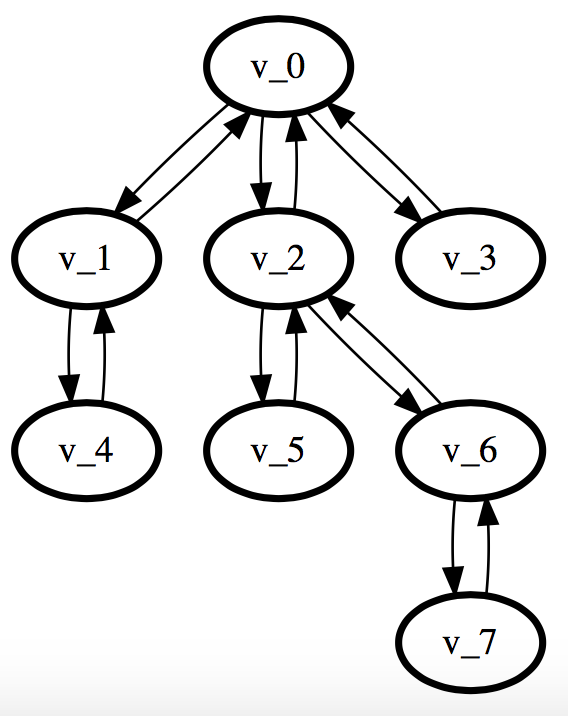
\includegraphics[width=2in]{1.png}

        \caption{Пример обхода остовного дерева,  построенного рассматриваемым алгоритмом.}
    \end{center}

    В результате обхода получим цикл  $C$, проходящий через все вершины. Очевидно, что $w(C) = 2w(MST)$, так как каждое ребро $MST$ входим в цикл дважды: в момент входа в поддерево и выхода из него. 

    Отсюда и из Леммы 1 получаем, что в графе $G$ есть гамильтонов цикл $\hat{C}$, причем $w(\hat{C}) \leq w(C) = 2w(MST)$, а доказательство леммы дает алгоритм для его поиска: оставить в $C$ только первые вхождения всех вершин. 

    Оценим приближение данного алгоритма:

    Пусть $\tilde{C}$ - гамильтонов цикл в $G$ минимального веса.
    Если из него убрать одно ребро то получим дерево, вес которого не меньше чем вес минимального остовного, то есть имеем соотношение $w(\tilde{C}) \geq w(MST) = \frac{w(C)}{2} \geq \frac{w(\hat{C})}{2}$ или $w(\hat{C}) \leq 2w(\tilde{C})$, то есть алгоритм действительно дает 2-приближение$.\Box$
    \paragraph{\large{5. $\frac{3}{2}$-приближение для метрической задачи}}\mbox{}\\
    Рассматриваемый алгоритм известен как алгоритм Кристофидеса[1].

    \textbf{Теорема 3} \textit{ Для метрической задачи коммивояжера существует полиномиальный алгоритм, дающий 1.5-приближение.}

    \textit{Доказательство}. Модифицируем предыдущий алгоритм:

    1) Аналогично построим $MST$.

    Рассмотрим полный подграф $H \subset G$, индуцированный на множестве вершин  $V_H = \{v | deg_{MST} v \equiv 1 (mod \quad 2)\}$.
    В $H$ четное число вершин, так как это число вершин с нечетной степенью в другом графе(дереве).

    2) Разобьем вершины  из $H$ на пары $M = {(v_0,v_1) ... (v_{k-1}, v_k)}$ таким образом, чтобы минимизировать сумму весов ребер в этих парах:

    \begin{equtation}
        \sum_{i=0}^{k/2} w(v_{2i},v_{2i+1}) \to min
    \end{equtation}

    Это можно сделать за полиномиальное время Венгерским алгоритмом о назначениях.

    Далее рассмотрим мультиграф $F = MST \cup M$.
    В нем все вершины имеют четную степень (так как $M$ добавило ребра в $MST$ к вершинам с нечетной степенью). 

    \begin{center} 
    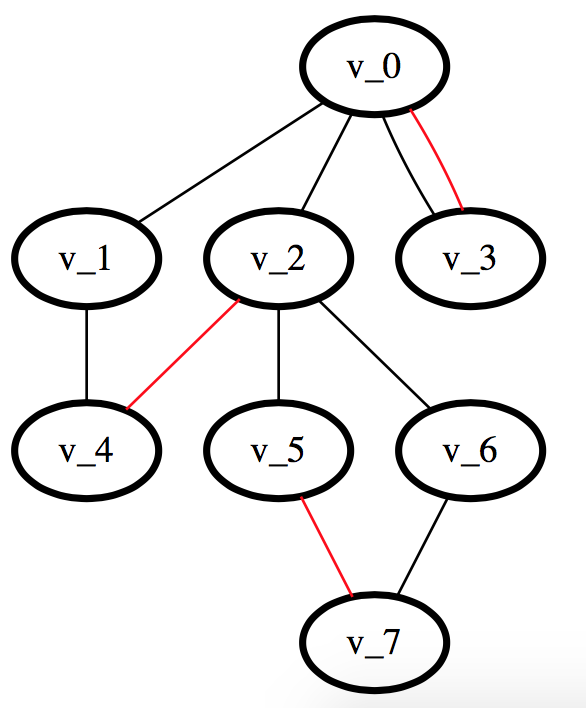
\includegraphics[width=2in]{2.png}

    \caption{Мультиграф $F$, полученный объединением $MST$ из предыдущего примера и паросочетания $M$ всех вершин с нечетной степенью в $MST$.}
    \end{center}

    Тогда в $F$ существует эйлеров цикл $C$, которому естественным образом соответствует цикл $\hat{C}$ в $G$, обходящий все вершины, причем $w(\hat{C}) = w(C)$. Значит по Лемме 1 в $G$ есть гамильтонов цикл $\tilde{C}$: $\tilde{C} \leq w(\hat{C} = w(C)$. 

    Можно оценить $\tilde{C} \leq w(\hat{C}) \leq w(MST) + w(M)$.
    Рассмотрим $\tilde{C}_M$ гамильтонов цикл  - ограничение $\tilde{C}$ на $M$ (выкинем из списка вершин $\tilde{C}$ все вершины не из $M$, оставшиеся вершины образуют гамильтонов цикл $V(M)$). 

    \begin{center} 
    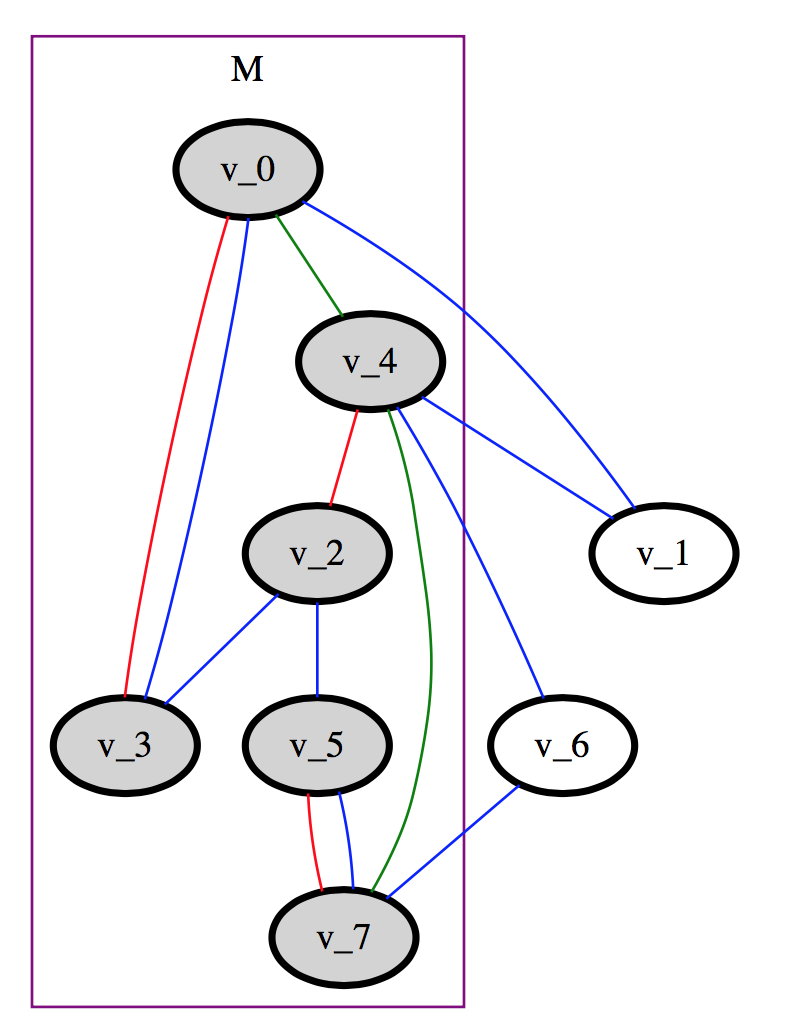
\includegraphics[width=2in]{4.png}

    \caption{Пример гамильтонова цикла $\tilde{C}$ в $G$ полученного алгоритмом в предыдущем примере(синий), паросочетания в $M$(красный) и ограничение $\tilde{C}_M$(зеленый и синий).}
    \end{center}

    Аналогично доказательству Леммы 1, по неравенству треугольника  $w(\tilde{C}_M) \leq w(\tilde{C})$. Но заметим, что $\tilde{C}_M$ - объединение двух непересекающихся паросочетаний в $V(M)$,  причем вес каждого из них не менее чем вес минимального паросочетания - $M$, а это значит, что $2w(M) \leq \tilde{C}_M \leq \tilde{C}$ или $w(M) \leq \frac{w(\tilde{C})}{2}$.

    Далее из доказательства Теоремы 2: $w(MST) \leq w(\tilde{C})$. 
    В итоге получаем, что $w(\hat{C}) \leq w(\tilde{C}) + \frac{w(\tilde{C})}{2} = 1.5 w(\tilde{C})$, то есть алгоритм действительно дает 1.5-приближение$.\Box$

  

    \paragraph{\large{6. Имплементация Алгоритма Кристофидеса}}\mbox{}\\

     Код на С++[2]

     Алгоритм состоит из 3 частей:

     1)  минимальное остовное дерево(алгоритм Крускала[3], 
     за $\mathcal{O}(NlogN)$).

     2) минимальное паросочетание в полном взвешенном неориентированном графе(Алгоритм Эдмунса сжатия цветков[4] за  $\mathcal{O}(N^2logN)$) .

     3) эйлеров цикл в неориенитированном мультиграфе(за $\mathcal{O}(N^2)$).

     Итоговая асимптотика - $\mathcal{O}(N^2logN)$.

     Для паросочетания была использована реализация автора статьи о быстром поиске этого паросочетания [4].

     Остальные части алгоритма протестированы отдельно в соответствующих задачах с онлайн контестов[5],[6].

     Алгоритм принимает на вход неориентированный взвешенный граф,  который дополняется до полного проведением недостающих ребер бесконечного веса.

     Входные веса проходят проверку на корректность метрики (то есть проверяются все неравенства треугольника).

     \newpage
     Корректность приближения алгоритма проверяется на специальных случайных тестах для которых известен правильный ответ.

     \begin{itemize}
     \item рассмотрим полный граф, в котором проведем случайно цикл по всем вершинам $V$ с ребрами веса 1, а вес остальных ребер выберем случайно: 1 или 2 (веса больше 2 не берем, чтобы точно сохранять неравенство треугольника)
    точный ответ - $|V|$

     \item рассмотрим специальную задачу поиска гамильтонова \textit{пути}[7].
     В частности с помощью этой задачи можно решить задачу поиска гамильтонова цикла в полном неориентированном графе. Для этого достаточно запустить поиск гамильтонова пути между всеми пар вершин и добавить ребро между ними к ответу, после чего взять минимум. Специальный граф описывается следующими условиями на ребра графа:
     \begin{enumerate}
     \item Вершинам графа $\{1,\dots|V|\}$ сопоставим их $'$координаты$'$ на прямой: $0 \leq x_1 \leq \dots \leq x_{|V|}$, 
     а также произовльные числа $a_i \geq 0$.
     \item Тогда вес ребра между $i$ и $j$ равен $|x_i - x_j| + a_i + a_j$
     \end{enumerate}
     Видно, что такой выбор весов удовлетворяет свойствам метрики.
     Для тестов просто сгенерируем случайные $a_i$ и $x_i$. Нахождение точного решения в данном случае работает за $\mathcal{O}(N^4)$.
     \end{itemize}
     Запустим оба теста несколько раз:

             \begin{center}
                    \begin{tabular}{|c|c|c|c|c|c|c|c|c|c|c|}
                            \hline 
                                $номер теста$ & 1 & 2 & 3 & 4 & 5 & 6 & 7 & 8 & 9 & 10 \\
                            \hline
                                тип теста &1 &1 &1 &1 &1 &2 &2 &2 &2 &2 \\
                            \hline
                                количество вершин &100 &100 &1000 &1000 &1000 &10 &100 &100 &100 &150 \\  
                            \hline 
                                точное решение &100 &100 &1000 &1000 &1000 &1664 &19604 &18866 &20076 &20802 \\
                            \hline
                                приближенное решение &124 &120 &1252 &1401 &1265 &1664 &19618 &18868 &20076 &20810 \\
                            \hline
                                ошибка &24\% &20\% &25\% &40\% &26\% &0\% &<0.01\% &<0.01\% &0\% &<0.01\%  \\
                    \end{tabular}
        \end{center}

        Как видно во всех случаях ошибка не превосходит заявленых $50\%$. Также интересно то, что на тестах 2 типа приближенный алгоритм дает практически верное решение.

        \paragraph{\large{7. Ссылки}}\mbox{}\\
        \begin{itemize}
        \item $[1]$ Christofides' Algorithm, Design and Analysis of Algorithms, Stanford University.

        \item $[2]$ \url{https://github.com/sergmiller/TSP1.5approx/tree/master/christofides/christofides}

        \item $[3]$ \url{https://en.wikipedia.org/wiki/Kruskal%27s_algorithm}

        \item $[4]$ Kolmogorov, V., Blossom V: a new implementation of a minimum cost perfect matching algorithm, Springer and Mathematical Programming Society, 2009.

        \item $[5]$ \url{http://informatics.mccme.ru/mod/statements/view.php?id=3580#1}

        \item $[6]$ \url{http://informatics.mccme.ru/moodle/mod/statements/view.php?chapterid=932#1}

        \item $[7]$ http://codeforces.com/contest/705/problem/D. 
        
        \end{itemize}
\end{document}
